\documentclass[14pt]{extbook}
\usepackage{multicol, enumerate, enumitem, hyperref, color, soul, setspace, parskip, fancyhdr} %General Packages
\usepackage{amssymb, amsthm, amsmath, bbm, latexsym, units, mathtools} %Math Packages
\everymath{\displaystyle} %All math in Display Style
% Packages with additional options
\usepackage[headsep=0.5cm,headheight=12pt, left=1 in,right= 1 in,top= 1 in,bottom= 1 in]{geometry}
\usepackage[usenames,dvipsnames]{xcolor}
\usepackage{dashrule}  % Package to use the command below to create lines between items
\newcommand{\litem}[1]{\item#1\hspace*{-1cm}\rule{\textwidth}{0.4pt}}
\pagestyle{fancy}
\lhead{Progress Quiz 4}
\chead{}
\rhead{Version C}
\lfoot{8448-1521}
\cfoot{}
\rfoot{Fall 2020}
\begin{document}

\begin{enumerate}
\litem{
Solve the radical equation below. Then, choose the interval(s) that the solution(s) belongs to.\[ \sqrt{-15 x^2 + 30} - \sqrt{15 x} = 0 \]\begin{enumerate}[label=\Alph*.]
\item \( x_1 \in [0, 2] \text{ and } x_2 \in [1.56,2.69] \)
\item \( x \in [0,2] \)
\item \( x \in [-6,-1] \)
\item \( x_1 \in [-6, -1] \text{ and } x_2 \in [0.72,1.17] \)
\item \( \text{All solutions lead to invalid or complex values in the equation.} \)

\end{enumerate} }
\litem{
Solve the radical equation below. Then, choose the interval(s) that the solution(s) belongs to.\[ \sqrt{-15 x^2 - 36} - \sqrt{-48 x} = 0 \]\begin{enumerate}[label=\Alph*.]
\item \( x_1 \in [0.96, 1.4] \text{ and } x_2 \in [2,3] \)
\item \( x \in [1.82,2.13] \)
\item \( x_1 \in [-1.3, -0.9] \text{ and } x_2 \in [-5,0] \)
\item \( x \in [0.96,1.4] \)
\item \( \text{All solutions lead to invalid or complex values in the equation.} \)

\end{enumerate} }
\litem{
What is the domain of the function below?\[ f(x) = \sqrt[6]{-6 x + 8} \]\begin{enumerate}[label=\Alph*.]
\item \( (-\infty, a], \text{where } a \in [0.59, 0.82] \)
\item \( (-\infty, \infty) \)
\item \( [a, \infty), \text{where } a \in [1.04, 2.01] \)
\item \( [a, \infty), \text{where } a \in [0.53, 1.15] \)
\item \( (-\infty, a], \text{ where } a \in [1.19, 1.4] \)

\end{enumerate} }
\litem{
Choose the graph of the equation below.\[ f(x) = \sqrt{x + 6} - 3 \]\begin{enumerate}[label=\Alph*.]
\begin{multicols}{2}\item 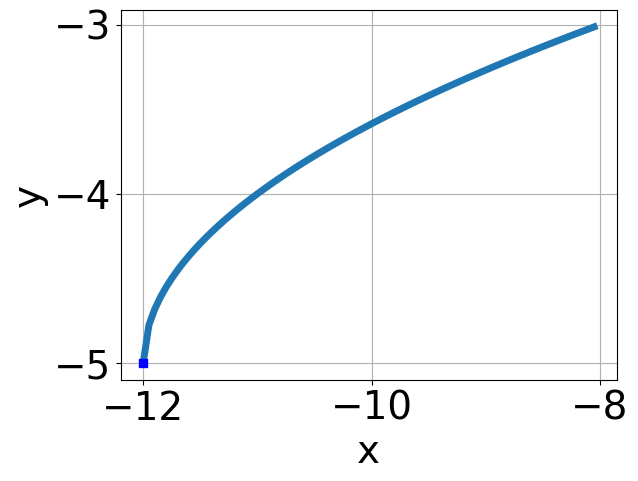
\includegraphics[width = 0.3\textwidth]{../Figures/radicalEquationToGraphAC.png}\item 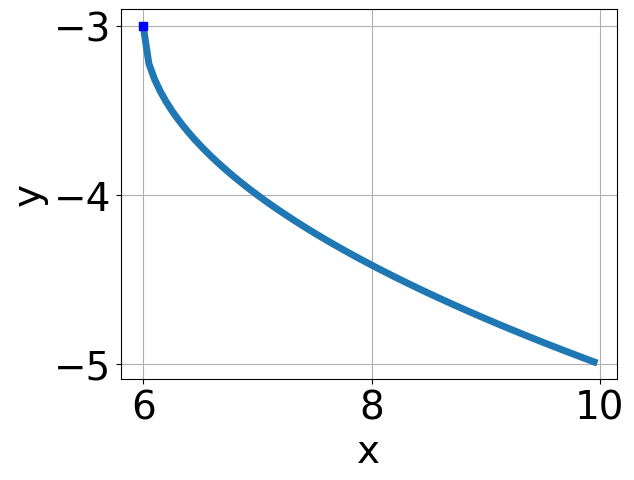
\includegraphics[width = 0.3\textwidth]{../Figures/radicalEquationToGraphBC.png}\item 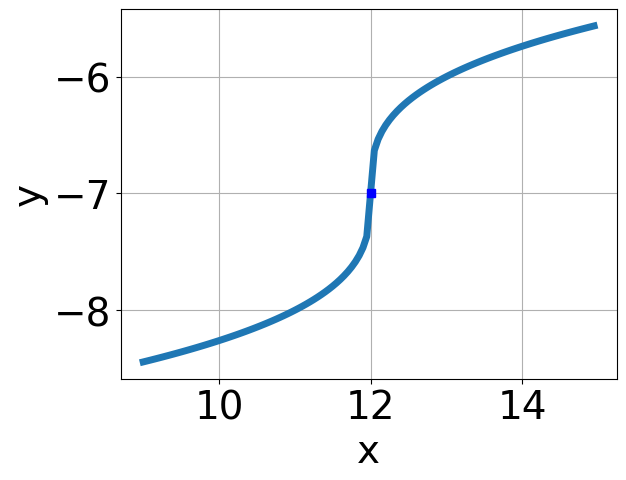
\includegraphics[width = 0.3\textwidth]{../Figures/radicalEquationToGraphCC.png}\item 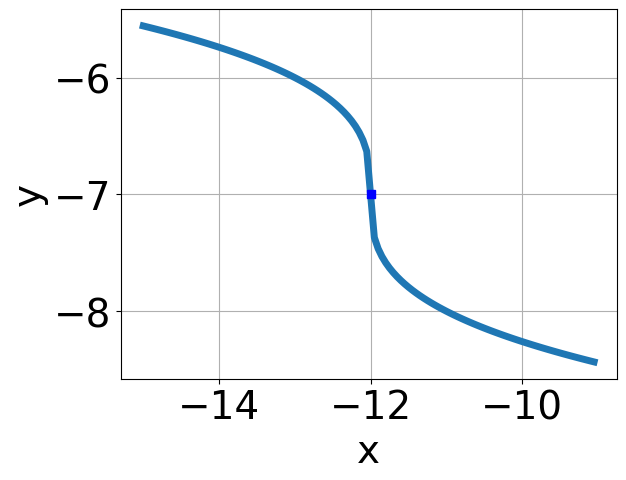
\includegraphics[width = 0.3\textwidth]{../Figures/radicalEquationToGraphDC.png}\end{multicols}\item None of the above.
\end{enumerate} }
\litem{
Choose the equation of the function graphed below.
\begin{center}
    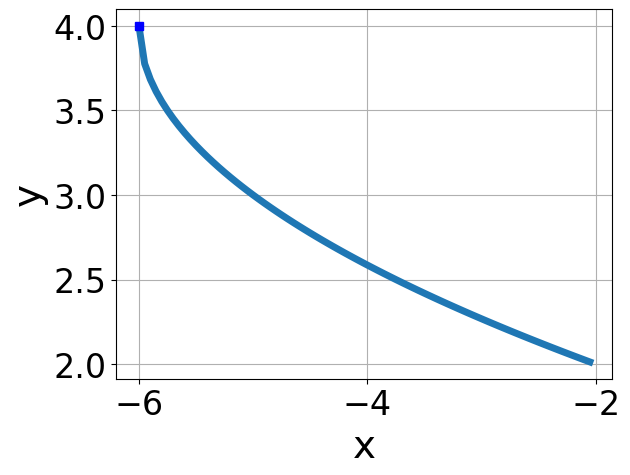
\includegraphics[width=0.5\textwidth]{../Figures/radicalGraphToEquationCopyC.png}
\end{center}
\begin{enumerate}[label=\Alph*.]
\item \( f(x) = \sqrt[3]{x + 14} - 5 \)
\item \( f(x) = - \sqrt[3]{x + 14} - 5 \)
\item \( f(x) = - \sqrt[3]{x - 14} - 5 \)
\item \( f(x) = \sqrt[3]{x - 14} - 5 \)
\item \( \text{None of the above} \)

\end{enumerate} }
\litem{
Solve the radical equation below. Then, choose the interval(s) that the solution(s) belongs to.\[ \sqrt{-5 x + 8} - \sqrt{8 x - 7} = 0 \]\begin{enumerate}[label=\Alph*.]
\item \( x_1 \in [0.7, 0.92] \text{ and } x_2 \in [-2.4,3.6] \)
\item \( \text{All solutions lead to invalid or complex values in the equation.} \)
\item \( x \in [1.04,1.35] \)
\item \( x_1 \in [1.04, 1.35] \text{ and } x_2 \in [-2.4,3.6] \)
\item \( x \in [-0.01,0.22] \)

\end{enumerate} }
\litem{
Choose the graph of the equation below.\[ f(x) = \sqrt{x + 12} + 3 \]\begin{enumerate}[label=\Alph*.]
\begin{multicols}{2}\item 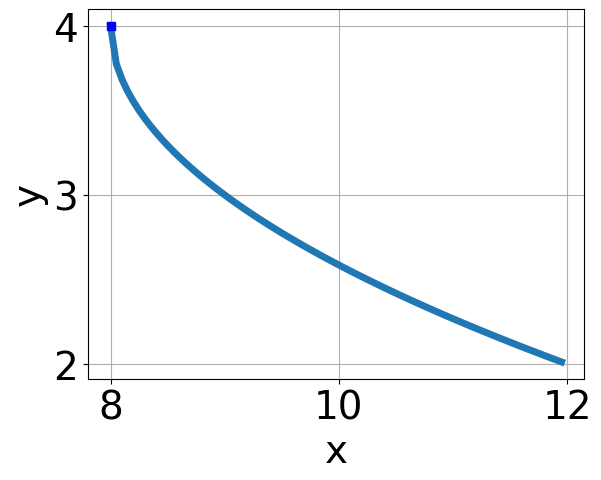
\includegraphics[width = 0.3\textwidth]{../Figures/radicalEquationToGraphCopyAC.png}\item 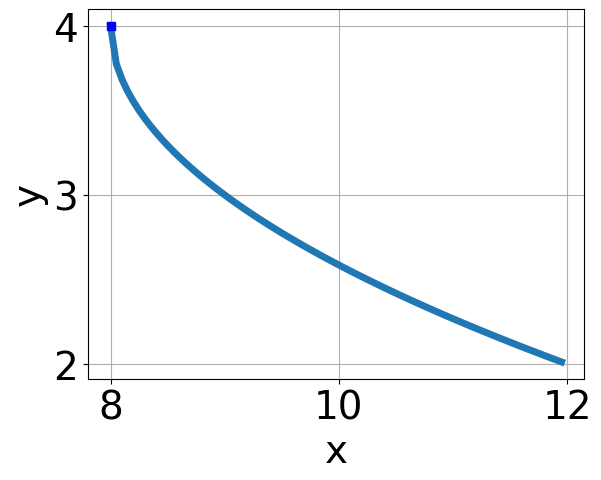
\includegraphics[width = 0.3\textwidth]{../Figures/radicalEquationToGraphCopyBC.png}\item 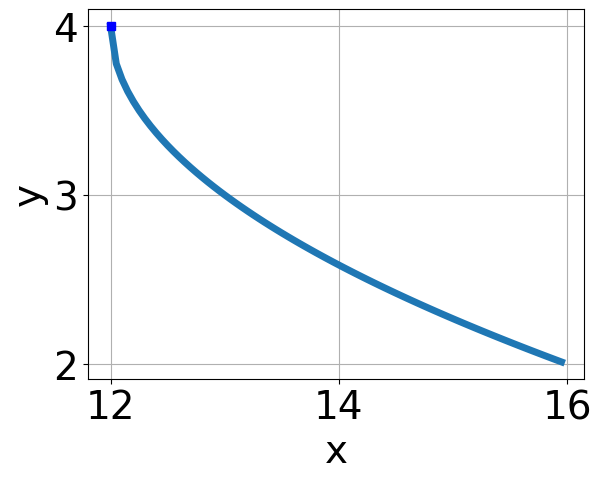
\includegraphics[width = 0.3\textwidth]{../Figures/radicalEquationToGraphCopyCC.png}\item 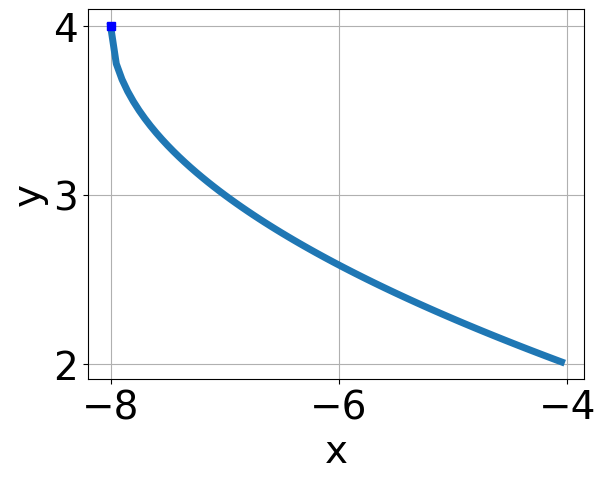
\includegraphics[width = 0.3\textwidth]{../Figures/radicalEquationToGraphCopyDC.png}\end{multicols}\item None of the above.
\end{enumerate} }
\litem{
Choose the equation of the function graphed below.
\begin{center}
    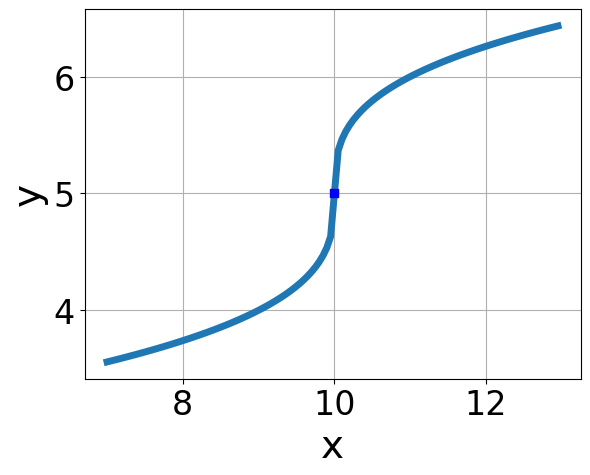
\includegraphics[width=0.5\textwidth]{../Figures/radicalGraphToEquationC.png}
\end{center}
\begin{enumerate}[label=\Alph*.]
\item \( f(x) = - \sqrt{x + 12} - 6 \)
\item \( f(x) = \sqrt{x + 12} - 6 \)
\item \( f(x) = \sqrt{x - 12} - 6 \)
\item \( f(x) = - \sqrt{x - 12} - 6 \)
\item \( \text{None of the above} \)

\end{enumerate} }
\litem{
Solve the radical equation below. Then, choose the interval(s) that the solution(s) belongs to.\[ \sqrt{-7 x + 5} - \sqrt{4 x + 7} = 0 \]\begin{enumerate}[label=\Alph*.]
\item \( x \in [-1.1,0.65] \)
\item \( x_1 \in [-1.1, 0.65] \text{ and } x_2 \in [-2.29,3.71] \)
\item \( x_1 \in [-2.03, -1.37] \text{ and } x_2 \in [-2.29,3.71] \)
\item \( x \in [0.19,1.58] \)
\item \( \text{All solutions lead to invalid or complex values in the equation.} \)

\end{enumerate} }
\litem{
What is the domain of the function below?\[ f(x) = \sqrt[4]{-3 x - 7} \]\begin{enumerate}[label=\Alph*.]
\item \( [a, \infty), \text{where } a \in [-3.62, -0.76] \)
\item \( [a, \infty), \text{where } a \in [-0.91, 1.29] \)
\item \( (-\infty, a], \text{ where } a \in [-3.3, -1.4] \)
\item \( (-\infty, a], \text{where } a \in [-2.1, 1.6] \)
\item \( (-\infty, \infty) \)

\end{enumerate} }
\end{enumerate}

\end{document}